\documentclass[a4paper,11pt,uplatex]{jsarticle}


% 数式
\usepackage{amsmath,amsfonts}
\usepackage{bm}
\usepackage{physics}
% 画像
\usepackage[dvipdfmx]{graphicx}
\usepackage[dvipdfmx,colorlinks=true,linkcolor=blue]{hyperref}
\usepackage{pxjahyper}

\begin{document}


\section{原理}
アンジュレータ放射光干渉法の概要を以下の図に示す。
初めにアンジュレータ放射光の発生原理と放射される放射光の性質を述べる。
続いて2台のアンジュレータを用いることによる干渉の原理を示す。軸上($\theta =0$)放射の場合と、一般の$\theta$におけるエネルギー決定公式を導く。
続いて放射光観測のための光学系による工学処理の原理を示す。
最後にこれらの原理をまとめた完全な物理モデルによる関数系の概要を示す。
\subsection{アンジュレータ放射光}
アンジュレータの原理を以下に示す。アンジュレータによって発生した周期的磁場中を電子ビームが通過すると、電子が蛇行("undulate")する。
磁場による加速度運動に伴いシンクロトロン放射光が発生する。
磁場周期と電子ビームエネルギーに依存して、発生する放射光は特定の波長に強いピークを持つ。
この特性はアンジュレータのK値と呼ばれる以下の特徴量によって表現できる。
$\text{K} \simeq 1$の時をアンジュレータと呼び準単色光が得られるが、$\text{K} \gg 1$の時には広い波長にわたって等間隔にピークを持つような放射光が発生し、このような挿入光源をウィグラーと呼ぶ。
アンジュレータ放射光の時間構造は以下に示すようなパルス型であることが知られている。
\subsubsection{アンジュレータ放射光 - タンデムアンジュレータ}
アンジュレータを電子ビームに沿って2つ連結した構成は放射光科学において広く使われている。
これらのアンジュレータ間にシケイン電磁石を配置することで遅延を調整することが可能になる。
\subsubsection{干渉の原理}
タンデム型アンジュレータから放射される放射光はダブルパルス型の波形となる。
回折格子のそれぞれの格子から散乱された光は格子間隔に比例して遅延された光の干渉となる。
そのためダブルパルスの二つのパルスは格子に寄る遅延を受けて干渉できることになる。
\subsubsection{電子ビームエネルギーと干渉光周期の関係式}
ダブルパルスの間隔は以下のような近似で理解することができる。
上流のアンジュレータで発生する放射光は電子ビームよりも早く、電子が下流側のアンジュレータに到達した時にはアンジュレータ間の距離に比例した時間差が生じる。
\begin{eqnarray}
  \Delta = \frac{1}{2\gamma^2}d \label{path shift}
\end{eqnarray}
この時間差は放射光の2つのパルスの位相差となる。
\begin{eqnarray}
  \Phi = 2\pi \frac{Delta}{\lambda_L}
\end{eqnarray}
位相差に対応して干渉光は強めあい、干渉光強度は
\begin{eqnarray}
  |\tilde{E} \left( 1+ e^{i\Phi}\right)|^2 
&= |\tilde{E}|^2 \left( 1 + \cos(\Phi) \right)\\
&= |\tilde{E}|^2 \left( 1 + \cos(\frac{2\pi}{2\gamma^2\lambda_L}d) \right) 
  \label{oscillation}
\end{eqnarray}
これより、dを変化させると干渉光の位相差が変化し強度が周期的に変動することがわかる。
式(\ref{oscillation})から、アンジュレータ間距離を$2\gamma^2\lambda_L$だけ動かした時に1周する。
この周期を$\lambda_{osc}$とおけば$\gamma$および電子ビームエネルギーが
\begin{eqnarray}
  \gamma = \sqrt{\frac{\lambda_{\text{osc}}}{2\lambda_L}}\\
  \text{E}_\text{beam} =m_e c^2  \sqrt{\frac{\lambda_{\text{osc}}}{2\lambda_L}} \label{zero order energy formula}
\end{eqnarray}
すなわち、干渉光の波長$\lambda_L$と、アンジュレータ間距離を変動させた時の干渉光の変動の周期$\lambda_{\text{osc}}$
を精密に測定することで電子ビームエネルギーが精密に測定できる。
\subsection{補正 - 放射角度と干渉光周期の関係式}
式(\ref*{path shift})は放射光角度が電子ビームの光路差である。
電子ビームの軸と放射光の放射角(近似的に放射光の観測角)を$\theta$とおくと、
アンジュレータ間の距離$d$と$\theta$で光路差が$d(1-\cos{\theta})$と表される。
これと電子ビームの遅延による光路差の両方を考慮した光路差は、
\begin{eqnarray}
  \Delta &= d\frac{1}{2\gamma^2} + d(1 - \cos{\theta}) \\
        &\sim d(\frac{1}{2\gamma^2} + \frac{\theta^2}{2})\\
\end{eqnarray}
と表せる。したがって放射光の観測角($\simeq$ 放射角)の補正を入れることで干渉光の周期は
\begin{eqnarray}
  \lambda_{\text{osc}} = \frac{\lambda_L}{\frac{1}{2\gamma^2} + \frac{\theta^2}{2}}
\end{eqnarray}
となる。


\subsection{光学系}
放射光は光学系を通してカメラで光学的に撮影する。光学系の役割は分光とパルス波形の平面化にある。
式(\ref{zero order energy formula})が示すとおり、
電子ビームエネルギーは波長に依存するため$10^{-4}$の絶対値較正精度を得るために波長決定精度は少なくとも$10^{-4}$程度必要となる。
またタンデムアンジュレータから放射される放射光は図、式(??)が示すようにダブルパルス型の波形を持ちこのままでは2つのパルスは干渉を起こさない。
そのため平面波化(フーリエ変換)が必要となる。
\begin{figure}[tb]
  \centering
  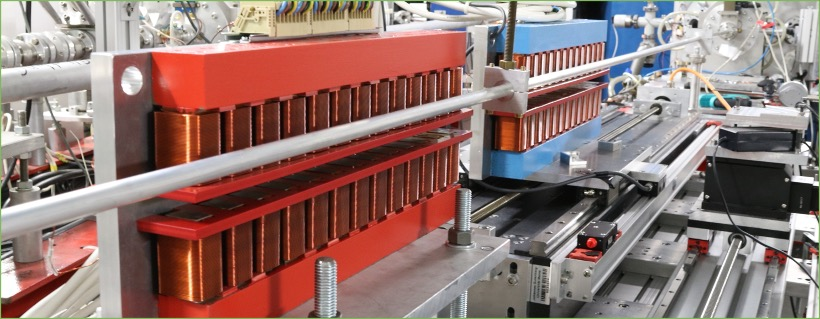
\includegraphics[width=0.8\linewidth]{image/1-1.jpg}\\
  \caption{サンプルの図}
  \label{optics_schematic}
\end{figure}
図\ref{optics_schematic}に光学系の概要を示す。
矩形スリットで整形した光波は伝搬に従って回折を生じる。後段には回折格子およびレンズがあり、
光波は分光と平面波化を受けカメラに到達する。
\subsubsection{レイリー・ゾンマーフェルト回折積分}
光波の伝搬はマクスウェル方程式に従う。
ある平面の波面から別の平面での波面を計算するには、レイリーゾンマーフェルト回折積分が知られている。
今回のセットアップにおいては近軸近似を用いることで、スクリーンでの回折パターンを式(??)によって計算できる。
数値計算手法については第3章に記述する。
\subsubsection{回折格子とレンズによる分光}
波面は回折格子で波長ごとに特定の方向に分光される。
レンズによって集光することでカメラでは特定の波長が鋭いピークとなるため、高い波長分解能を実現できる。
\subsubsection{回折格子による平面波化}

\subsubsection{撮影画像}
これらの一連の流れを図(??)に示した。
回折格子による分光、平面波化作用は水平方向にのみ作用する。従って画像の横軸は波長に対応し、縦軸の座標は観測角に対応する。
\subsection{モデル関数}
モデル関数の概要を示す。
放射光関数は、電子ビームとアンジュレータのパラメータを入力としてスリット直前の入射光の振幅および位相を計算する。
光学関数は、入射光の位相と振幅を入力としてスクリーンにおける回折光の振幅を計算する。
撮影画像を再現する最も確からしいパラメータの組を求めることで、電子ビームのエネルギーが決定できる。


\clearpage

\begin{figure}[tb]
  \centering
  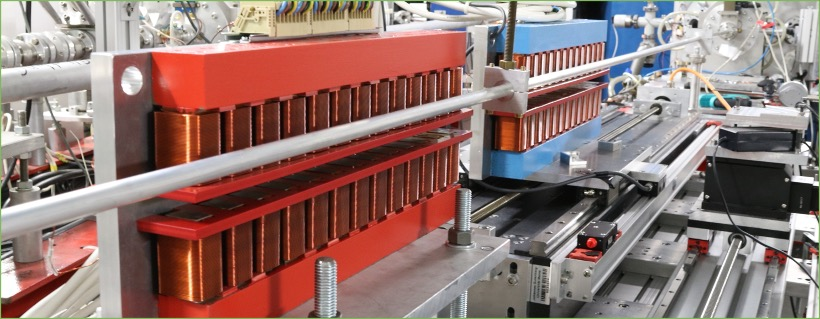
\includegraphics[width=0.8\linewidth]{image/1-1.jpg}\\
  \caption{サンプルの図}
  \label{sample_image}
\end{figure}

\begin{itemize}
  \item a
\end{itemize}
\begin{enumerate}
  \item b
\end{enumerate}

\begin{align}
\frac{1}{2} = \qty(\frac{1}{3}) + \qty{1}\Sigma
\end{align}
\end{document}
